\documentclass[11pt]{article}

    \usepackage[breakable]{tcolorbox}
    \usepackage{parskip} % Stop auto-indenting (to mimic markdown behaviour)
    
    \usepackage{iftex}
    \ifPDFTeX
    	\usepackage[T1]{fontenc}
    	\usepackage{mathpazo}
    \else
    	\usepackage{fontspec}
    \fi

    % Basic figure setup, for now with no caption control since it's done
    % automatically by Pandoc (which extracts ![](path) syntax from Markdown).
    \usepackage{graphicx}
    % Maintain compatibility with old templates. Remove in nbconvert 6.0
    \let\Oldincludegraphics\includegraphics
    % Ensure that by default, figures have no caption (until we provide a
    % proper Figure object with a Caption API and a way to capture that
    % in the conversion process - todo).
    \usepackage{caption}
    \DeclareCaptionFormat{nocaption}{}
    \captionsetup{format=nocaption,aboveskip=0pt,belowskip=0pt}

    \usepackage[Export]{adjustbox} % Used to constrain images to a maximum size
    \adjustboxset{max size={0.9\linewidth}{0.9\paperheight}}
    \usepackage{float}
    \floatplacement{figure}{H} % forces figures to be placed at the correct location
    \usepackage{xcolor} % Allow colors to be defined
    \usepackage{enumerate} % Needed for markdown enumerations to work
    \usepackage{geometry} % Used to adjust the document margins
    \usepackage{amsmath} % Equations
    \usepackage{amssymb} % Equations
    \usepackage{textcomp} % defines textquotesingle
    % Hack from http://tex.stackexchange.com/a/47451/13684:
    \AtBeginDocument{%
        \def\PYZsq{\textquotesingle}% Upright quotes in Pygmentized code
    }
    \usepackage{upquote} % Upright quotes for verbatim code
    \usepackage{eurosym} % defines \euro
    \usepackage[mathletters]{ucs} % Extended unicode (utf-8) support
    \usepackage{fancyvrb} % verbatim replacement that allows latex
    \usepackage{grffile} % extends the file name processing of package graphics 
                         % to support a larger range
    \makeatletter % fix for grffile with XeLaTeX
    \def\Gread@@xetex#1{%
      \IfFileExists{"\Gin@base".bb}%
      {\Gread@eps{\Gin@base.bb}}%
      {\Gread@@xetex@aux#1}%
    }
    \makeatother

    % The hyperref package gives us a pdf with properly built
    % internal navigation ('pdf bookmarks' for the table of contents,
    % internal cross-reference links, web links for URLs, etc.)
    \usepackage{hyperref}
    % The default LaTeX title has an obnoxious amount of whitespace. By default,
    % titling removes some of it. It also provides customization options.
    \usepackage{titling}
    \usepackage{longtable} % longtable support required by pandoc >1.10
    \usepackage{booktabs}  % table support for pandoc > 1.12.2
    \usepackage[inline]{enumitem} % IRkernel/repr support (it uses the enumerate* environment)
    \usepackage[normalem]{ulem} % ulem is needed to support strikethroughs (\sout)
                                % normalem makes italics be italics, not underlines
    \usepackage{mathrsfs}
    

    
    % Colors for the hyperref package
    \definecolor{urlcolor}{rgb}{0,.145,.698}
    \definecolor{linkcolor}{rgb}{.71,0.21,0.01}
    \definecolor{citecolor}{rgb}{.12,.54,.11}

    % ANSI colors
    \definecolor{ansi-black}{HTML}{3E424D}
    \definecolor{ansi-black-intense}{HTML}{282C36}
    \definecolor{ansi-red}{HTML}{E75C58}
    \definecolor{ansi-red-intense}{HTML}{B22B31}
    \definecolor{ansi-green}{HTML}{00A250}
    \definecolor{ansi-green-intense}{HTML}{007427}
    \definecolor{ansi-yellow}{HTML}{DDB62B}
    \definecolor{ansi-yellow-intense}{HTML}{B27D12}
    \definecolor{ansi-blue}{HTML}{208FFB}
    \definecolor{ansi-blue-intense}{HTML}{0065CA}
    \definecolor{ansi-magenta}{HTML}{D160C4}
    \definecolor{ansi-magenta-intense}{HTML}{A03196}
    \definecolor{ansi-cyan}{HTML}{60C6C8}
    \definecolor{ansi-cyan-intense}{HTML}{258F8F}
    \definecolor{ansi-white}{HTML}{C5C1B4}
    \definecolor{ansi-white-intense}{HTML}{A1A6B2}
    \definecolor{ansi-default-inverse-fg}{HTML}{FFFFFF}
    \definecolor{ansi-default-inverse-bg}{HTML}{000000}

    % commands and environments needed by pandoc snippets
    % extracted from the output of `pandoc -s`
    \providecommand{\tightlist}{%
      \setlength{\itemsep}{0pt}\setlength{\parskip}{0pt}}
    \DefineVerbatimEnvironment{Highlighting}{Verbatim}{commandchars=\\\{\}}
    % Add ',fontsize=\small' for more characters per line
    \newenvironment{Shaded}{}{}
    \newcommand{\KeywordTok}[1]{\textcolor[rgb]{0.00,0.44,0.13}{\textbf{{#1}}}}
    \newcommand{\DataTypeTok}[1]{\textcolor[rgb]{0.56,0.13,0.00}{{#1}}}
    \newcommand{\DecValTok}[1]{\textcolor[rgb]{0.25,0.63,0.44}{{#1}}}
    \newcommand{\BaseNTok}[1]{\textcolor[rgb]{0.25,0.63,0.44}{{#1}}}
    \newcommand{\FloatTok}[1]{\textcolor[rgb]{0.25,0.63,0.44}{{#1}}}
    \newcommand{\CharTok}[1]{\textcolor[rgb]{0.25,0.44,0.63}{{#1}}}
    \newcommand{\StringTok}[1]{\textcolor[rgb]{0.25,0.44,0.63}{{#1}}}
    \newcommand{\CommentTok}[1]{\textcolor[rgb]{0.38,0.63,0.69}{\textit{{#1}}}}
    \newcommand{\OtherTok}[1]{\textcolor[rgb]{0.00,0.44,0.13}{{#1}}}
    \newcommand{\AlertTok}[1]{\textcolor[rgb]{1.00,0.00,0.00}{\textbf{{#1}}}}
    \newcommand{\FunctionTok}[1]{\textcolor[rgb]{0.02,0.16,0.49}{{#1}}}
    \newcommand{\RegionMarkerTok}[1]{{#1}}
    \newcommand{\ErrorTok}[1]{\textcolor[rgb]{1.00,0.00,0.00}{\textbf{{#1}}}}
    \newcommand{\NormalTok}[1]{{#1}}
    
    % Additional commands for more recent versions of Pandoc
    \newcommand{\ConstantTok}[1]{\textcolor[rgb]{0.53,0.00,0.00}{{#1}}}
    \newcommand{\SpecialCharTok}[1]{\textcolor[rgb]{0.25,0.44,0.63}{{#1}}}
    \newcommand{\VerbatimStringTok}[1]{\textcolor[rgb]{0.25,0.44,0.63}{{#1}}}
    \newcommand{\SpecialStringTok}[1]{\textcolor[rgb]{0.73,0.40,0.53}{{#1}}}
    \newcommand{\ImportTok}[1]{{#1}}
    \newcommand{\DocumentationTok}[1]{\textcolor[rgb]{0.73,0.13,0.13}{\textit{{#1}}}}
    \newcommand{\AnnotationTok}[1]{\textcolor[rgb]{0.38,0.63,0.69}{\textbf{\textit{{#1}}}}}
    \newcommand{\CommentVarTok}[1]{\textcolor[rgb]{0.38,0.63,0.69}{\textbf{\textit{{#1}}}}}
    \newcommand{\VariableTok}[1]{\textcolor[rgb]{0.10,0.09,0.49}{{#1}}}
    \newcommand{\ControlFlowTok}[1]{\textcolor[rgb]{0.00,0.44,0.13}{\textbf{{#1}}}}
    \newcommand{\OperatorTok}[1]{\textcolor[rgb]{0.40,0.40,0.40}{{#1}}}
    \newcommand{\BuiltInTok}[1]{{#1}}
    \newcommand{\ExtensionTok}[1]{{#1}}
    \newcommand{\PreprocessorTok}[1]{\textcolor[rgb]{0.74,0.48,0.00}{{#1}}}
    \newcommand{\AttributeTok}[1]{\textcolor[rgb]{0.49,0.56,0.16}{{#1}}}
    \newcommand{\InformationTok}[1]{\textcolor[rgb]{0.38,0.63,0.69}{\textbf{\textit{{#1}}}}}
    \newcommand{\WarningTok}[1]{\textcolor[rgb]{0.38,0.63,0.69}{\textbf{\textit{{#1}}}}}
    
    
    % Define a nice break command that doesn't care if a line doesn't already
    % exist.
    \def\br{\hspace*{\fill} \\* }
    % Math Jax compatibility definitions
    \def\gt{>}
    \def\lt{<}
    \let\Oldtex\TeX
    \let\Oldlatex\LaTeX
    \renewcommand{\TeX}{\textrm{\Oldtex}}
    \renewcommand{\LaTeX}{\textrm{\Oldlatex}}
    % Document parameters
    % Document title
    \title{Day II - Part III - GitLab CI}
    
    
    
    
    
% Pygments definitions
\makeatletter
\def\PY@reset{\let\PY@it=\relax \let\PY@bf=\relax%
    \let\PY@ul=\relax \let\PY@tc=\relax%
    \let\PY@bc=\relax \let\PY@ff=\relax}
\def\PY@tok#1{\csname PY@tok@#1\endcsname}
\def\PY@toks#1+{\ifx\relax#1\empty\else%
    \PY@tok{#1}\expandafter\PY@toks\fi}
\def\PY@do#1{\PY@bc{\PY@tc{\PY@ul{%
    \PY@it{\PY@bf{\PY@ff{#1}}}}}}}
\def\PY#1#2{\PY@reset\PY@toks#1+\relax+\PY@do{#2}}

\expandafter\def\csname PY@tok@w\endcsname{\def\PY@tc##1{\textcolor[rgb]{0.73,0.73,0.73}{##1}}}
\expandafter\def\csname PY@tok@c\endcsname{\let\PY@it=\textit\def\PY@tc##1{\textcolor[rgb]{0.25,0.50,0.50}{##1}}}
\expandafter\def\csname PY@tok@cp\endcsname{\def\PY@tc##1{\textcolor[rgb]{0.74,0.48,0.00}{##1}}}
\expandafter\def\csname PY@tok@k\endcsname{\let\PY@bf=\textbf\def\PY@tc##1{\textcolor[rgb]{0.00,0.50,0.00}{##1}}}
\expandafter\def\csname PY@tok@kp\endcsname{\def\PY@tc##1{\textcolor[rgb]{0.00,0.50,0.00}{##1}}}
\expandafter\def\csname PY@tok@kt\endcsname{\def\PY@tc##1{\textcolor[rgb]{0.69,0.00,0.25}{##1}}}
\expandafter\def\csname PY@tok@o\endcsname{\def\PY@tc##1{\textcolor[rgb]{0.40,0.40,0.40}{##1}}}
\expandafter\def\csname PY@tok@ow\endcsname{\let\PY@bf=\textbf\def\PY@tc##1{\textcolor[rgb]{0.67,0.13,1.00}{##1}}}
\expandafter\def\csname PY@tok@nb\endcsname{\def\PY@tc##1{\textcolor[rgb]{0.00,0.50,0.00}{##1}}}
\expandafter\def\csname PY@tok@nf\endcsname{\def\PY@tc##1{\textcolor[rgb]{0.00,0.00,1.00}{##1}}}
\expandafter\def\csname PY@tok@nc\endcsname{\let\PY@bf=\textbf\def\PY@tc##1{\textcolor[rgb]{0.00,0.00,1.00}{##1}}}
\expandafter\def\csname PY@tok@nn\endcsname{\let\PY@bf=\textbf\def\PY@tc##1{\textcolor[rgb]{0.00,0.00,1.00}{##1}}}
\expandafter\def\csname PY@tok@ne\endcsname{\let\PY@bf=\textbf\def\PY@tc##1{\textcolor[rgb]{0.82,0.25,0.23}{##1}}}
\expandafter\def\csname PY@tok@nv\endcsname{\def\PY@tc##1{\textcolor[rgb]{0.10,0.09,0.49}{##1}}}
\expandafter\def\csname PY@tok@no\endcsname{\def\PY@tc##1{\textcolor[rgb]{0.53,0.00,0.00}{##1}}}
\expandafter\def\csname PY@tok@nl\endcsname{\def\PY@tc##1{\textcolor[rgb]{0.63,0.63,0.00}{##1}}}
\expandafter\def\csname PY@tok@ni\endcsname{\let\PY@bf=\textbf\def\PY@tc##1{\textcolor[rgb]{0.60,0.60,0.60}{##1}}}
\expandafter\def\csname PY@tok@na\endcsname{\def\PY@tc##1{\textcolor[rgb]{0.49,0.56,0.16}{##1}}}
\expandafter\def\csname PY@tok@nt\endcsname{\let\PY@bf=\textbf\def\PY@tc##1{\textcolor[rgb]{0.00,0.50,0.00}{##1}}}
\expandafter\def\csname PY@tok@nd\endcsname{\def\PY@tc##1{\textcolor[rgb]{0.67,0.13,1.00}{##1}}}
\expandafter\def\csname PY@tok@s\endcsname{\def\PY@tc##1{\textcolor[rgb]{0.73,0.13,0.13}{##1}}}
\expandafter\def\csname PY@tok@sd\endcsname{\let\PY@it=\textit\def\PY@tc##1{\textcolor[rgb]{0.73,0.13,0.13}{##1}}}
\expandafter\def\csname PY@tok@si\endcsname{\let\PY@bf=\textbf\def\PY@tc##1{\textcolor[rgb]{0.73,0.40,0.53}{##1}}}
\expandafter\def\csname PY@tok@se\endcsname{\let\PY@bf=\textbf\def\PY@tc##1{\textcolor[rgb]{0.73,0.40,0.13}{##1}}}
\expandafter\def\csname PY@tok@sr\endcsname{\def\PY@tc##1{\textcolor[rgb]{0.73,0.40,0.53}{##1}}}
\expandafter\def\csname PY@tok@ss\endcsname{\def\PY@tc##1{\textcolor[rgb]{0.10,0.09,0.49}{##1}}}
\expandafter\def\csname PY@tok@sx\endcsname{\def\PY@tc##1{\textcolor[rgb]{0.00,0.50,0.00}{##1}}}
\expandafter\def\csname PY@tok@m\endcsname{\def\PY@tc##1{\textcolor[rgb]{0.40,0.40,0.40}{##1}}}
\expandafter\def\csname PY@tok@gh\endcsname{\let\PY@bf=\textbf\def\PY@tc##1{\textcolor[rgb]{0.00,0.00,0.50}{##1}}}
\expandafter\def\csname PY@tok@gu\endcsname{\let\PY@bf=\textbf\def\PY@tc##1{\textcolor[rgb]{0.50,0.00,0.50}{##1}}}
\expandafter\def\csname PY@tok@gd\endcsname{\def\PY@tc##1{\textcolor[rgb]{0.63,0.00,0.00}{##1}}}
\expandafter\def\csname PY@tok@gi\endcsname{\def\PY@tc##1{\textcolor[rgb]{0.00,0.63,0.00}{##1}}}
\expandafter\def\csname PY@tok@gr\endcsname{\def\PY@tc##1{\textcolor[rgb]{1.00,0.00,0.00}{##1}}}
\expandafter\def\csname PY@tok@ge\endcsname{\let\PY@it=\textit}
\expandafter\def\csname PY@tok@gs\endcsname{\let\PY@bf=\textbf}
\expandafter\def\csname PY@tok@gp\endcsname{\let\PY@bf=\textbf\def\PY@tc##1{\textcolor[rgb]{0.00,0.00,0.50}{##1}}}
\expandafter\def\csname PY@tok@go\endcsname{\def\PY@tc##1{\textcolor[rgb]{0.53,0.53,0.53}{##1}}}
\expandafter\def\csname PY@tok@gt\endcsname{\def\PY@tc##1{\textcolor[rgb]{0.00,0.27,0.87}{##1}}}
\expandafter\def\csname PY@tok@err\endcsname{\def\PY@bc##1{\setlength{\fboxsep}{0pt}\fcolorbox[rgb]{1.00,0.00,0.00}{1,1,1}{\strut ##1}}}
\expandafter\def\csname PY@tok@kc\endcsname{\let\PY@bf=\textbf\def\PY@tc##1{\textcolor[rgb]{0.00,0.50,0.00}{##1}}}
\expandafter\def\csname PY@tok@kd\endcsname{\let\PY@bf=\textbf\def\PY@tc##1{\textcolor[rgb]{0.00,0.50,0.00}{##1}}}
\expandafter\def\csname PY@tok@kn\endcsname{\let\PY@bf=\textbf\def\PY@tc##1{\textcolor[rgb]{0.00,0.50,0.00}{##1}}}
\expandafter\def\csname PY@tok@kr\endcsname{\let\PY@bf=\textbf\def\PY@tc##1{\textcolor[rgb]{0.00,0.50,0.00}{##1}}}
\expandafter\def\csname PY@tok@bp\endcsname{\def\PY@tc##1{\textcolor[rgb]{0.00,0.50,0.00}{##1}}}
\expandafter\def\csname PY@tok@fm\endcsname{\def\PY@tc##1{\textcolor[rgb]{0.00,0.00,1.00}{##1}}}
\expandafter\def\csname PY@tok@vc\endcsname{\def\PY@tc##1{\textcolor[rgb]{0.10,0.09,0.49}{##1}}}
\expandafter\def\csname PY@tok@vg\endcsname{\def\PY@tc##1{\textcolor[rgb]{0.10,0.09,0.49}{##1}}}
\expandafter\def\csname PY@tok@vi\endcsname{\def\PY@tc##1{\textcolor[rgb]{0.10,0.09,0.49}{##1}}}
\expandafter\def\csname PY@tok@vm\endcsname{\def\PY@tc##1{\textcolor[rgb]{0.10,0.09,0.49}{##1}}}
\expandafter\def\csname PY@tok@sa\endcsname{\def\PY@tc##1{\textcolor[rgb]{0.73,0.13,0.13}{##1}}}
\expandafter\def\csname PY@tok@sb\endcsname{\def\PY@tc##1{\textcolor[rgb]{0.73,0.13,0.13}{##1}}}
\expandafter\def\csname PY@tok@sc\endcsname{\def\PY@tc##1{\textcolor[rgb]{0.73,0.13,0.13}{##1}}}
\expandafter\def\csname PY@tok@dl\endcsname{\def\PY@tc##1{\textcolor[rgb]{0.73,0.13,0.13}{##1}}}
\expandafter\def\csname PY@tok@s2\endcsname{\def\PY@tc##1{\textcolor[rgb]{0.73,0.13,0.13}{##1}}}
\expandafter\def\csname PY@tok@sh\endcsname{\def\PY@tc##1{\textcolor[rgb]{0.73,0.13,0.13}{##1}}}
\expandafter\def\csname PY@tok@s1\endcsname{\def\PY@tc##1{\textcolor[rgb]{0.73,0.13,0.13}{##1}}}
\expandafter\def\csname PY@tok@mb\endcsname{\def\PY@tc##1{\textcolor[rgb]{0.40,0.40,0.40}{##1}}}
\expandafter\def\csname PY@tok@mf\endcsname{\def\PY@tc##1{\textcolor[rgb]{0.40,0.40,0.40}{##1}}}
\expandafter\def\csname PY@tok@mh\endcsname{\def\PY@tc##1{\textcolor[rgb]{0.40,0.40,0.40}{##1}}}
\expandafter\def\csname PY@tok@mi\endcsname{\def\PY@tc##1{\textcolor[rgb]{0.40,0.40,0.40}{##1}}}
\expandafter\def\csname PY@tok@il\endcsname{\def\PY@tc##1{\textcolor[rgb]{0.40,0.40,0.40}{##1}}}
\expandafter\def\csname PY@tok@mo\endcsname{\def\PY@tc##1{\textcolor[rgb]{0.40,0.40,0.40}{##1}}}
\expandafter\def\csname PY@tok@ch\endcsname{\let\PY@it=\textit\def\PY@tc##1{\textcolor[rgb]{0.25,0.50,0.50}{##1}}}
\expandafter\def\csname PY@tok@cm\endcsname{\let\PY@it=\textit\def\PY@tc##1{\textcolor[rgb]{0.25,0.50,0.50}{##1}}}
\expandafter\def\csname PY@tok@cpf\endcsname{\let\PY@it=\textit\def\PY@tc##1{\textcolor[rgb]{0.25,0.50,0.50}{##1}}}
\expandafter\def\csname PY@tok@c1\endcsname{\let\PY@it=\textit\def\PY@tc##1{\textcolor[rgb]{0.25,0.50,0.50}{##1}}}
\expandafter\def\csname PY@tok@cs\endcsname{\let\PY@it=\textit\def\PY@tc##1{\textcolor[rgb]{0.25,0.50,0.50}{##1}}}

\def\PYZbs{\char`\\}
\def\PYZus{\char`\_}
\def\PYZob{\char`\{}
\def\PYZcb{\char`\}}
\def\PYZca{\char`\^}
\def\PYZam{\char`\&}
\def\PYZlt{\char`\<}
\def\PYZgt{\char`\>}
\def\PYZsh{\char`\#}
\def\PYZpc{\char`\%}
\def\PYZdl{\char`\$}
\def\PYZhy{\char`\-}
\def\PYZsq{\char`\'}
\def\PYZdq{\char`\"}
\def\PYZti{\char`\~}
% for compatibility with earlier versions
\def\PYZat{@}
\def\PYZlb{[}
\def\PYZrb{]}
\makeatother


    % For linebreaks inside Verbatim environment from package fancyvrb. 
    \makeatletter
        \newbox\Wrappedcontinuationbox 
        \newbox\Wrappedvisiblespacebox 
        \newcommand*\Wrappedvisiblespace {\textcolor{red}{\textvisiblespace}} 
        \newcommand*\Wrappedcontinuationsymbol {\textcolor{red}{\llap{\tiny$\m@th\hookrightarrow$}}} 
        \newcommand*\Wrappedcontinuationindent {3ex } 
        \newcommand*\Wrappedafterbreak {\kern\Wrappedcontinuationindent\copy\Wrappedcontinuationbox} 
        % Take advantage of the already applied Pygments mark-up to insert 
        % potential linebreaks for TeX processing. 
        %        {, <, #, %, $, ' and ": go to next line. 
        %        _, }, ^, &, >, - and ~: stay at end of broken line. 
        % Use of \textquotesingle for straight quote. 
        \newcommand*\Wrappedbreaksatspecials {% 
            \def\PYGZus{\discretionary{\char`\_}{\Wrappedafterbreak}{\char`\_}}% 
            \def\PYGZob{\discretionary{}{\Wrappedafterbreak\char`\{}{\char`\{}}% 
            \def\PYGZcb{\discretionary{\char`\}}{\Wrappedafterbreak}{\char`\}}}% 
            \def\PYGZca{\discretionary{\char`\^}{\Wrappedafterbreak}{\char`\^}}% 
            \def\PYGZam{\discretionary{\char`\&}{\Wrappedafterbreak}{\char`\&}}% 
            \def\PYGZlt{\discretionary{}{\Wrappedafterbreak\char`\<}{\char`\<}}% 
            \def\PYGZgt{\discretionary{\char`\>}{\Wrappedafterbreak}{\char`\>}}% 
            \def\PYGZsh{\discretionary{}{\Wrappedafterbreak\char`\#}{\char`\#}}% 
            \def\PYGZpc{\discretionary{}{\Wrappedafterbreak\char`\%}{\char`\%}}% 
            \def\PYGZdl{\discretionary{}{\Wrappedafterbreak\char`\$}{\char`\$}}% 
            \def\PYGZhy{\discretionary{\char`\-}{\Wrappedafterbreak}{\char`\-}}% 
            \def\PYGZsq{\discretionary{}{\Wrappedafterbreak\textquotesingle}{\textquotesingle}}% 
            \def\PYGZdq{\discretionary{}{\Wrappedafterbreak\char`\"}{\char`\"}}% 
            \def\PYGZti{\discretionary{\char`\~}{\Wrappedafterbreak}{\char`\~}}% 
        } 
        % Some characters . , ; ? ! / are not pygmentized. 
        % This macro makes them "active" and they will insert potential linebreaks 
        \newcommand*\Wrappedbreaksatpunct {% 
            \lccode`\~`\.\lowercase{\def~}{\discretionary{\hbox{\char`\.}}{\Wrappedafterbreak}{\hbox{\char`\.}}}% 
            \lccode`\~`\,\lowercase{\def~}{\discretionary{\hbox{\char`\,}}{\Wrappedafterbreak}{\hbox{\char`\,}}}% 
            \lccode`\~`\;\lowercase{\def~}{\discretionary{\hbox{\char`\;}}{\Wrappedafterbreak}{\hbox{\char`\;}}}% 
            \lccode`\~`\:\lowercase{\def~}{\discretionary{\hbox{\char`\:}}{\Wrappedafterbreak}{\hbox{\char`\:}}}% 
            \lccode`\~`\?\lowercase{\def~}{\discretionary{\hbox{\char`\?}}{\Wrappedafterbreak}{\hbox{\char`\?}}}% 
            \lccode`\~`\!\lowercase{\def~}{\discretionary{\hbox{\char`\!}}{\Wrappedafterbreak}{\hbox{\char`\!}}}% 
            \lccode`\~`\/\lowercase{\def~}{\discretionary{\hbox{\char`\/}}{\Wrappedafterbreak}{\hbox{\char`\/}}}% 
            \catcode`\.\active
            \catcode`\,\active 
            \catcode`\;\active
            \catcode`\:\active
            \catcode`\?\active
            \catcode`\!\active
            \catcode`\/\active 
            \lccode`\~`\~ 	
        }
    \makeatother

    \let\OriginalVerbatim=\Verbatim
    \makeatletter
    \renewcommand{\Verbatim}[1][1]{%
        %\parskip\z@skip
        \sbox\Wrappedcontinuationbox {\Wrappedcontinuationsymbol}%
        \sbox\Wrappedvisiblespacebox {\FV@SetupFont\Wrappedvisiblespace}%
        \def\FancyVerbFormatLine ##1{\hsize\linewidth
            \vtop{\raggedright\hyphenpenalty\z@\exhyphenpenalty\z@
                \doublehyphendemerits\z@\finalhyphendemerits\z@
                \strut ##1\strut}%
        }%
        % If the linebreak is at a space, the latter will be displayed as visible
        % space at end of first line, and a continuation symbol starts next line.
        % Stretch/shrink are however usually zero for typewriter font.
        \def\FV@Space {%
            \nobreak\hskip\z@ plus\fontdimen3\font minus\fontdimen4\font
            \discretionary{\copy\Wrappedvisiblespacebox}{\Wrappedafterbreak}
            {\kern\fontdimen2\font}%
        }%
        
        % Allow breaks at special characters using \PYG... macros.
        \Wrappedbreaksatspecials
        % Breaks at punctuation characters . , ; ? ! and / need catcode=\active 	
        \OriginalVerbatim[#1,codes*=\Wrappedbreaksatpunct]%
    }
    \makeatother

    % Exact colors from NB
    \definecolor{incolor}{HTML}{303F9F}
    \definecolor{outcolor}{HTML}{D84315}
    \definecolor{cellborder}{HTML}{CFCFCF}
    \definecolor{cellbackground}{HTML}{F7F7F7}
    
    % prompt
    \makeatletter
    \newcommand{\boxspacing}{\kern\kvtcb@left@rule\kern\kvtcb@boxsep}
    \makeatother
    \newcommand{\prompt}[4]{
        \ttfamily\llap{{\color{#2}[#3]:\hspace{3pt}#4}}\vspace{-\baselineskip}
    }
    

    
    % Prevent overflowing lines due to hard-to-break entities
    \sloppy 
    % Setup hyperref package
    \hypersetup{
      breaklinks=true,  % so long urls are correctly broken across lines
      colorlinks=true,
      urlcolor=urlcolor,
      linkcolor=linkcolor,
      citecolor=citecolor,
      }
    % Slightly bigger margins than the latex defaults
    
    \geometry{verbose,tmargin=1in,bmargin=1in,lmargin=1in,rmargin=1in}
    
    

\begin{document}
    
    \maketitle
    
    

    
    \hypertarget{continuous-integration-in-gitlab}{%
\section{Continuous integration in
gitlab}\label{continuous-integration-in-gitlab}}

    This part will demonstrate how to add automated building and testing to
your gitlab repository. This is also known as continuous integration or
CI.

    In the
\href{https://gitlab.gwdg.de/glynatsi/rsd-workshop/-/blob/master/Day\%20II\%20-\%20Part\%20II\%20-\%20GitLab\%20exercise.ipynb}{previous
part}, we have shown how to run your tests with \texttt{pytest}. Now we
will go one step further and instruct gitlab to run the test \emph{every
time} a change is committed to the code base.

    Detailed information about CI in gitlab can be found in the official
gitlab documentation at https://docs.gitlab.com/ee/ci/. Here we only
cover the basic steps to setup CI for your project.

    We will repeatedly mention the \texttt{repository\ root\ directory}.
This is the top level directory of the \texttt{distances} project,
i.e.~the directory that was created when we cloned the repository with
the \texttt{git\ clone} command. Make sure you change into the
repository root directory before following the instructions.

    \hypertarget{activate-ci-through-the-.gitlab-ci.yml-file.}{%
\subsection{\texorpdfstring{Activate CI through the
\texttt{.gitlab-ci.yml}
file.}{Activate CI through the .gitlab-ci.yml file.}}\label{activate-ci-through-the-.gitlab-ci.yml-file.}}

Gitlab automatically scans the root directory for a file named
\texttt{.gitlab-ci.yml}. If that file is detected, gitlab will parse
this file and execute the instructions. The file must follow the
\href{https://yaml.org}{\texttt{yaml} (``Yet Another Markup Language'')
syntax}.

    On the front page of your gitlab repo, click on \texttt{Setup\ CI/CD}

\begin{figure}
\centering
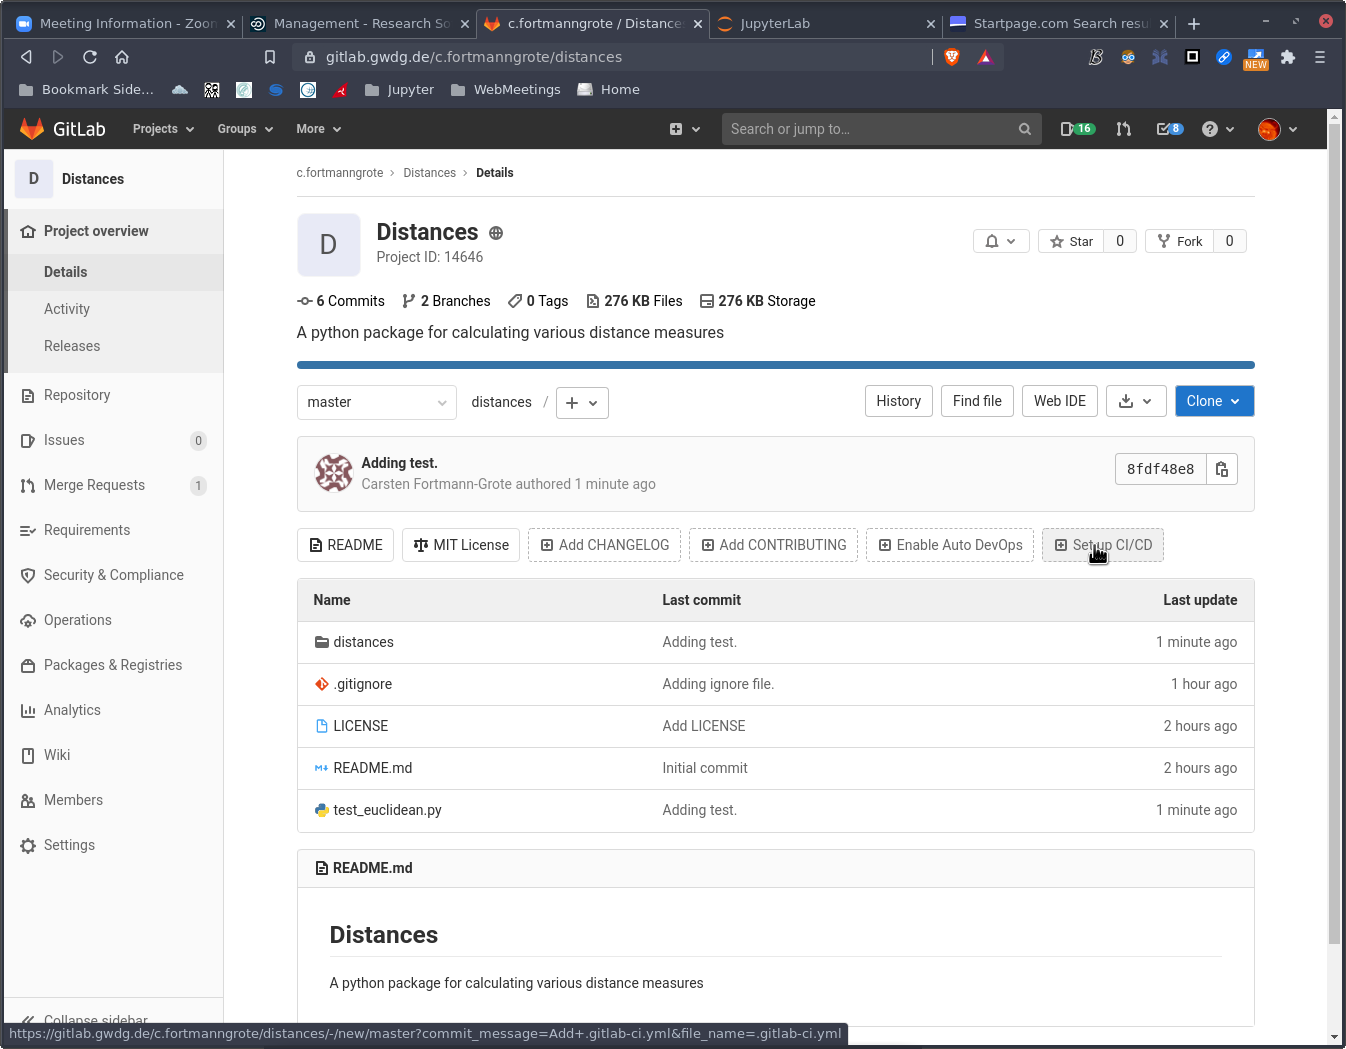
\includegraphics{static/distance_project.png}
\caption{Screenshot\_2020-12-07\_16-58-30.png}
\end{figure}

    Paste the following lines into the text entry field:

\begin{Shaded}
\begin{Highlighting}[]
\CommentTok{\# gitlab{-}ci yaml file for project "distances"}
\CommentTok{\# The docker base image to use.}
\FunctionTok{image}\KeywordTok{:}\AttributeTok{ python:latest}

\CommentTok{\# Run these commands before any jobs.}
\FunctionTok{before\_script}\KeywordTok{:}
\AttributeTok{  }\KeywordTok{{-}}\AttributeTok{ python {-}V}\CommentTok{                 \# Print out python version for debugging}
\AttributeTok{  }\KeywordTok{{-}}\AttributeTok{ pip install virtualenv}\CommentTok{    \# Pip install dependencies}
\AttributeTok{  }\KeywordTok{{-}}\AttributeTok{ virtualenv venv}\CommentTok{           \# Create }
\AttributeTok{  }\KeywordTok{{-}}\AttributeTok{ source venv/bin/activate}\CommentTok{  \# Activate the virtual environment.}
\AttributeTok{  }\KeywordTok{{-}}\AttributeTok{ pip install pytest}\CommentTok{        \# Install pytest into the venv.}

\CommentTok{\# The test job }
\FunctionTok{test}\KeywordTok{:}
\AttributeTok{  }\FunctionTok{script}\KeywordTok{:}
\AttributeTok{    }\KeywordTok{{-}}\AttributeTok{ pytest test\_euclidean.py}
\end{Highlighting}
\end{Shaded}

This \texttt{yml} file is structured as follows: * The ``base image'':
Gitlab-CI uses \href{https://docker.io}{docker} images to encapsulate
the test environment. * \texttt{before\_script}: Contains commands to
execute before any \texttt{jobs} are run. * \texttt{test}: The
\texttt{test} job runs the test code through pytest. * More jobs can be
defined.

    \textbf{Q:} Commit your changes using \texttt{git\ add} and
\texttt{git\ commit}.

Return to the gitlab repository front page and navigate to
\texttt{Settings} in the left navigation panel. Expand the second item
``Visibility, \ldots{}'' and activate the toggle named ``Pipelines''.

\begin{figure}
\centering
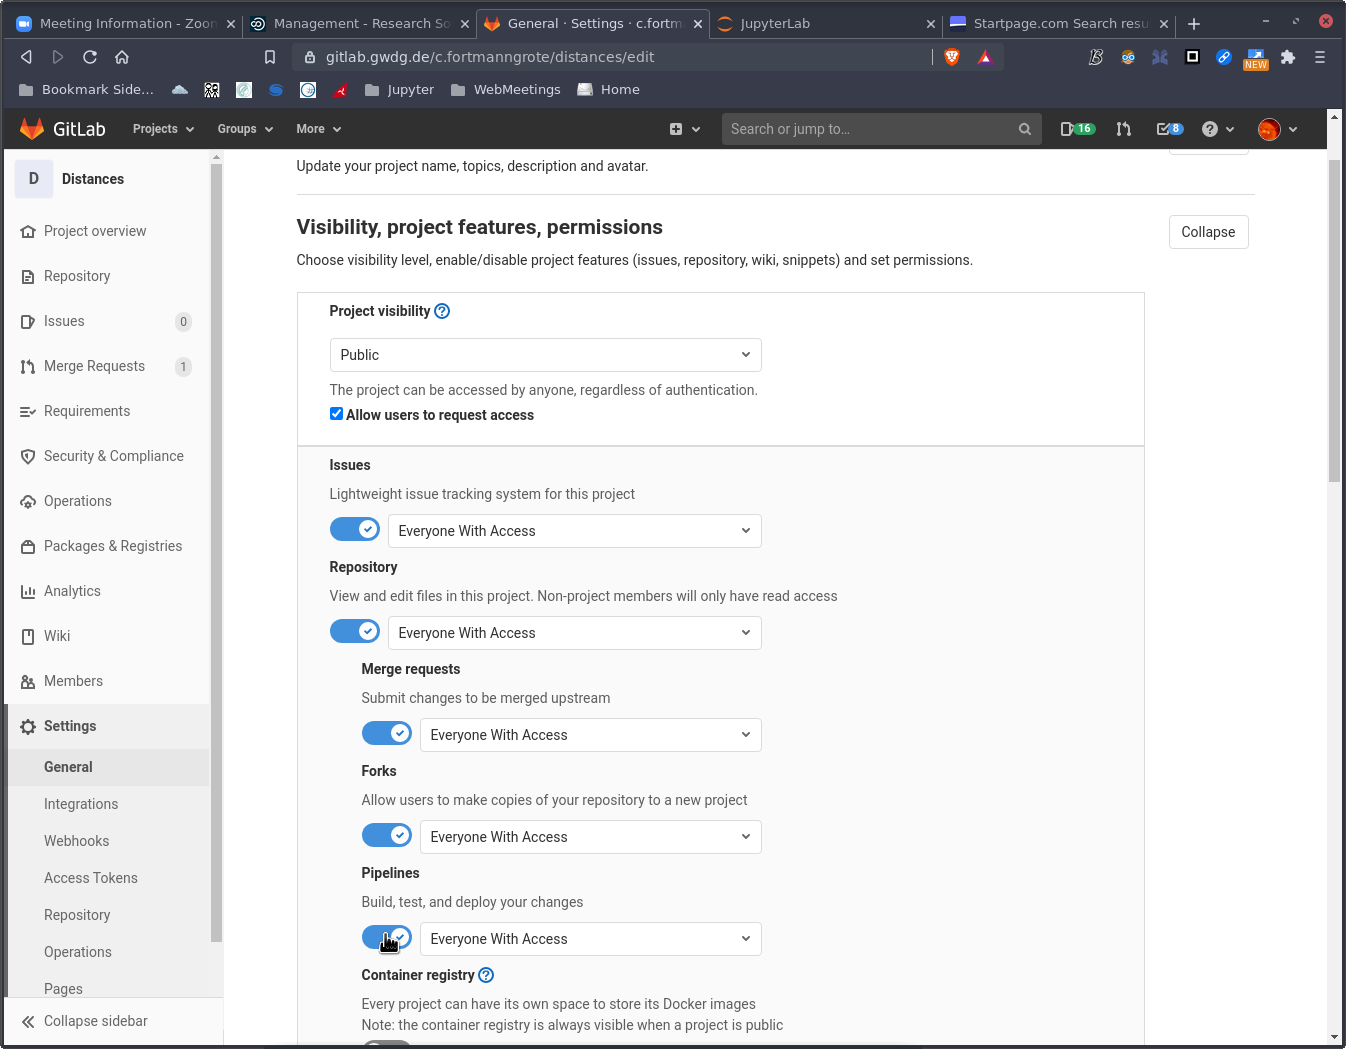
\includegraphics{static/settings.png}
\caption{Screenshot\_2020-12-07\_17-06-04.png}
\end{figure}

    Don't forget to click \texttt{Save\ changes} at the bottom of the page.

    You can now initialize a first CI run by navigating to \texttt{CI/CD} in
the left navigation panel, then click \texttt{Run\ pipeline} on the next
two pages.

After the test is finished, you will see a test report page, similar to
this one (it will look differently if the test failed\ldots)

\begin{figure}
\centering
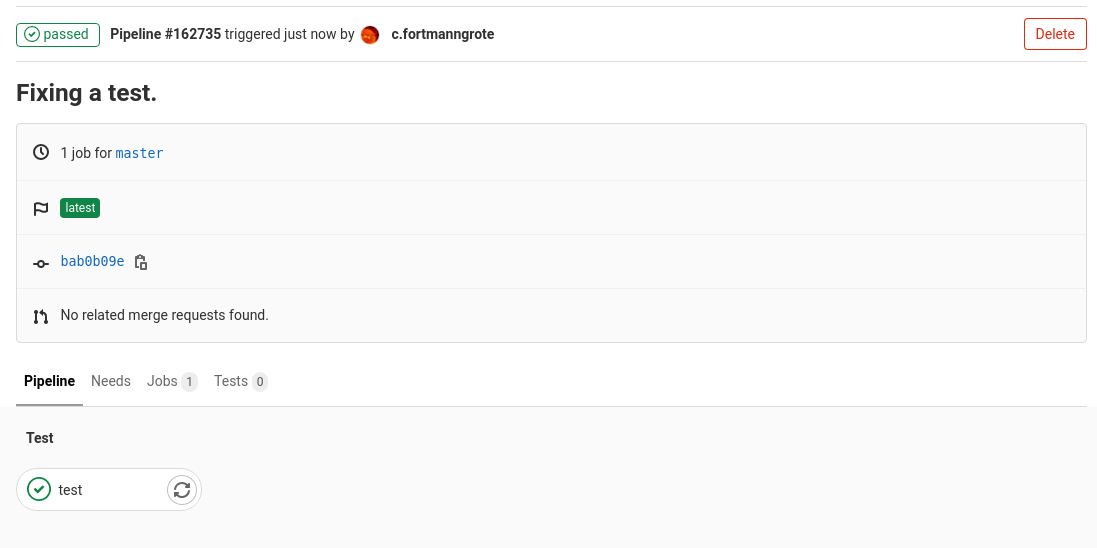
\includegraphics{static/CI.png}
\caption{Screenshot\_2020-12-07\_20-40-16.png}
\end{figure}

    Now let's try out the automated test feature. We will implement an
additional distance, the Manhattan distance. But this time, we'll do it
the pro way: We will \emph{first} add a test function for the new
distance metric. Naturally, the test will fail. Subsequently, we will
implement the new distance such that the test passes. This approach is
called \emph{test driven development} and is an established technique in
software engineering. The value of writing the test first is that we
have to get a very clear idea of the expected behaviour of our new
function, even before we start implementing it. If we were given a list
of requirements from our supervisor, we could add a test function for
each requirement and then implement the code such that one test after
the other succeeds. In the end, all requirements would be satisfied.

    \hypertarget{adding-the-new-test.}{%
\subsection{Adding the new test.}\label{adding-the-new-test.}}

We will add the new test module named \texttt{test\_manhattan.py} file.
Let's copy the file \texttt{test\_euclidean.py} and make the required
changes in the new file.

\begin{verbatim}
$ cp -v test_euclidean.py test_manhattan.py
\end{verbatim}

\textbf{Q:} What is the effect of the ``-v'' flag in the previous
command?

    Edit the new file \texttt{test\_manhattan.py} as follows

\begin{Shaded}
\begin{Highlighting}[]
\CommentTok{\# test\_manhattan.py}

\ImportTok{import}\NormalTok{ distances}

\KeywordTok{def}\NormalTok{ test\_manhattan():}
    \CommentTok{""" Test the manhattan distance calculation. """}
\NormalTok{    u }\OperatorTok{=}\NormalTok{ (}\DecValTok{2}\NormalTok{, }\OperatorTok{{-}}\DecValTok{1}\NormalTok{)}
\NormalTok{    v }\OperatorTok{=}\NormalTok{ (}\OperatorTok{{-}}\DecValTok{2}\NormalTok{, }\DecValTok{2}\NormalTok{)}

    \ControlFlowTok{assert}\NormalTok{ distances.manhattan\_distance(u, v) }\OperatorTok{==} \FloatTok{7.0}
\end{Highlighting}
\end{Shaded}

    Run the test and observe the test failure.

\begin{verbatim}
$ pytest test_manhattan.py
\end{verbatim}

    As expected, the test will fail because the \texttt{distances} package
has no definition of the \texttt{manhattan\_distance()} function that is
called in the \texttt{test\_manhattan} test function.

    \hypertarget{implement-the-new-distance-function.}{%
\subsection{Implement the new distance
function.}\label{implement-the-new-distance-function.}}

We implement the Manhattan distance in a new python module
\texttt{manhattan.py} in the package directory \texttt{distances/}:

\begin{Shaded}
\begin{Highlighting}[]
\CommentTok{\# distances/manhattan.py}
\ImportTok{import}\NormalTok{ math }

\KeywordTok{def}\NormalTok{ manhattan\_distance(u, v):}
    \CommentTok{"""}
\CommentTok{    Computes the Manhattan distance between two vectors \textasciigrave{}u\textasciigrave{} and \textasciigrave{}v\textasciigrave{}.}

\CommentTok{    The Euclidean distance between \textasciigrave{}u\textasciigrave{} and \textasciigrave{}v\textasciigrave{}, is defined as:}

\CommentTok{    |u\_1 {-} v\_1| + ... + |u\_n {-} v\_n|}

\CommentTok{    Parameters}
\CommentTok{    {-}{-}{-}{-}{-}{-}{-}{-}{-}{-}}
\CommentTok{    u : list}
\CommentTok{        Input vector.}
\CommentTok{    v : list}
\CommentTok{        Input vector.}

\CommentTok{    Returns}
\CommentTok{    {-}{-}{-}{-}{-}{-}{-}}
\CommentTok{    manhattan : double}
\CommentTok{        The Manhattan distance between vectors \textasciigrave{}u\textasciigrave{} and \textasciigrave{}v\textasciigrave{}.}
\CommentTok{    """}
\NormalTok{    distance }\OperatorTok{=} \DecValTok{0}

    \ControlFlowTok{for}\NormalTok{ u\_i, v\_i }\KeywordTok{in} \BuiltInTok{zip}\NormalTok{(u, v):}
\NormalTok{        distance }\OperatorTok{+=} \BuiltInTok{abs}\NormalTok{(u\_i }\OperatorTok{{-}}\NormalTok{ v\_i)}\OperatorTok{**}\DecValTok{2}

    \ControlFlowTok{return}\NormalTok{ distance}
\end{Highlighting}
\end{Shaded}

    Since we do not want to commit to master directly, we will create a new
branch:

\begin{verbatim}
$ git checkout -b implement_manhattan_distance
\end{verbatim}

\textbf{Q:} Note that the ``-b'' flag allows us to create and checkout
the new branch in one go.

Add the two new files and one modified file to git:

\begin{verbatim}
$ git add test_manhattan.py
$ git add distances/manhattan.py
$ git add distances/__init__.py
\end{verbatim}

And commit the changes:

\begin{verbatim}
$ git commit -m "Add manhattan distance and test."
\end{verbatim}

\textbf{Q:} What is the function of the ``-m'' flag in the
\texttt{git\ commit} command above?

    \hypertarget{register-the-new-test-module-to-ci}{%
\subsection{Register the new test module to
CI}\label{register-the-new-test-module-to-ci}}

Finally, we have to register the new test to the CI system. Edit the
file \texttt{.gitlab-ci.yml} as follows:

\begin{Shaded}
\begin{Highlighting}[]
\CommentTok{\# gitlab{-}ci yaml file for project "distances"}
\CommentTok{\# The docker base image to use.}
\FunctionTok{image}\KeywordTok{:}\AttributeTok{ python:latest}

\CommentTok{\# Run these commands before any jobs.}
\FunctionTok{before\_script}\KeywordTok{:}
\AttributeTok{  }\KeywordTok{{-}}\AttributeTok{ python {-}V}\CommentTok{                 \# Print out python version for debugging}
\AttributeTok{  }\KeywordTok{{-}}\AttributeTok{ pip install virtualenv}\CommentTok{    \# Pip install dependencies}
\AttributeTok{  }\KeywordTok{{-}}\AttributeTok{ virtualenv venv}\CommentTok{           \# Create }
\AttributeTok{  }\KeywordTok{{-}}\AttributeTok{ source venv/bin/activate}\CommentTok{  \# Activate the virtual environment.}
\AttributeTok{  }\KeywordTok{{-}}\AttributeTok{ pip install pytest}\CommentTok{        \# Install pytest into the venv.}

\CommentTok{\# The test job }
\FunctionTok{test}\KeywordTok{:}
\AttributeTok{  }\FunctionTok{script}\KeywordTok{:}
\AttributeTok{    }\KeywordTok{{-}}\AttributeTok{ pytest test\_euclidean.py}
\AttributeTok{    }\KeywordTok{{-}}\AttributeTok{ pytest test\_manhattan.py}
\end{Highlighting}
\end{Shaded}

    Add and commit this change:

\begin{verbatim}
$ git add .gitlab-ci.
$ git commit
\end{verbatim}

and push all changes to the remote branch on gitlab:

\begin{verbatim}
$ git push -u origin implement_manhattan_distance
\end{verbatim}

    \hypertarget{check-test-status-on-gitlab}{%
\subsection{Check test status on
gitlab}\label{check-test-status-on-gitlab}}

Now open your repository website and navigate to the CI summary page
(click CI/CD in the navigation panel).

\begin{figure}
\centering
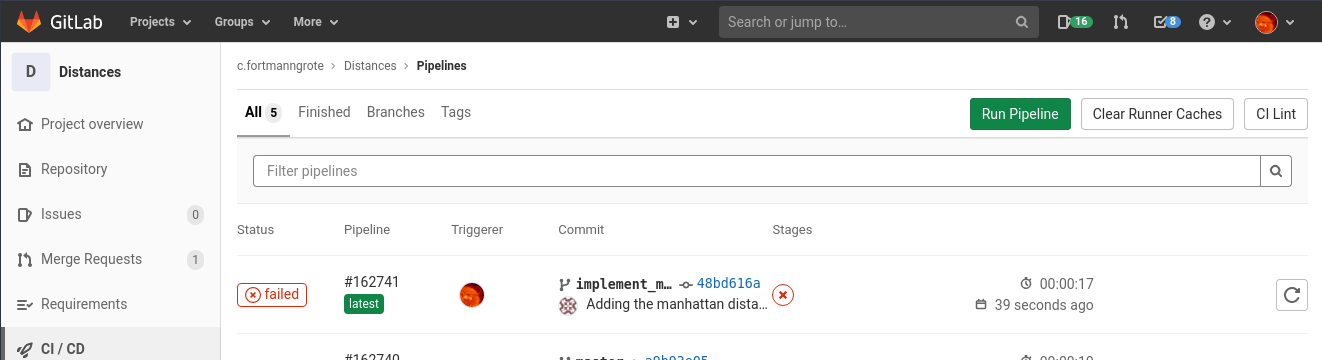
\includegraphics{static/test_gitlab.png}
\caption{Screenshot\_2020-12-07\_21-19-22.png}
\end{figure}

\textbf{What? The test failed!}

    Inspecting the test report, we find that the expected result and the
result our code gave, do not agree:

\begin{figure}
\centering
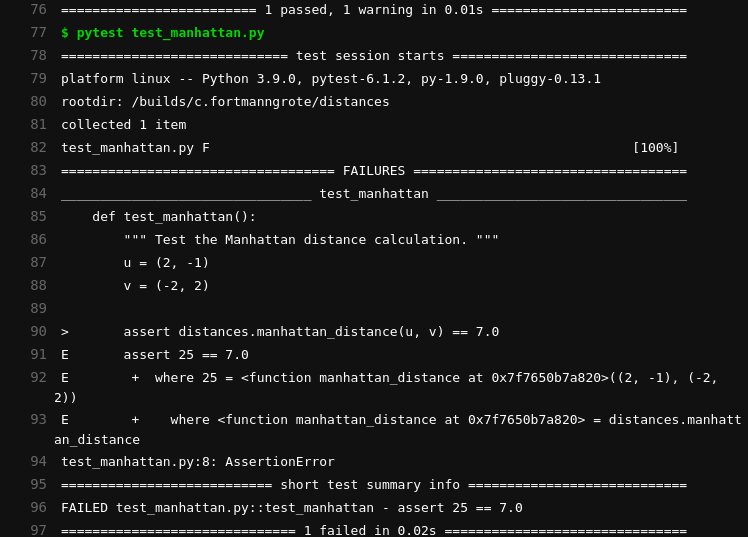
\includegraphics{static/failure_gitlab.png}
\caption{Screenshot\_2020-12-07\_21-28-30.png}
\end{figure}

    \textbf{Q:} Try to spot the error in \texttt{distances/manhattan.py} and
fix it. Then recommit to the repository and observe the test run.
Iterate this procedure until the test goes through.

    \hypertarget{building-the-documentation}{%
\section{Building the documentation}\label{building-the-documentation}}

The CI feature of gitlab not only allows us to run tests. In the
\texttt{.gitlab-ci.yml}, we can define any number of ``jobs'' that will
be run sequentially in a ``pipeline''. Typically, a complete CI pipeline
consists of * Installing dependencies * Building the code * Running the
tests * Building the documentation * Prepare a software package for the
users to download

    Here, we will demonstrate how to build a reference manual for our code.

The reference manual will be built based on the information we put into
the docstrings of our functions in our python modules. Take a look at
\texttt{distances/euclidean.py}:

\begin{Shaded}
\begin{Highlighting}[]
\CommentTok{\# distances/euclidean.py}

\ImportTok{import}\NormalTok{ math }

\KeywordTok{def}\NormalTok{ euclidean\_distance(u, v):}
    \CommentTok{"""}
\CommentTok{    Computes the Euclidean distance between two vectors \textasciigrave{}u\textasciigrave{} and \textasciigrave{}v\textasciigrave{}.}

\CommentTok{    The Euclidean distance between \textasciigrave{}u\textasciigrave{} and \textasciigrave{}v\textasciigrave{}, is defined as:}

\CommentTok{    \textbackslash{}sqrt\{(u\_1 {-} v\_1) \^{} 2 + ... + (u\_n {-} v\_n) \^{} 2\}}

\CommentTok{    Parameters}
\CommentTok{    {-}{-}{-}{-}{-}{-}{-}{-}{-}{-}}
\CommentTok{    u : list}
\CommentTok{        Input vector.}
\CommentTok{    v : list}
\CommentTok{        Input vector.}

\CommentTok{    Returns}
\CommentTok{    {-}{-}{-}{-}{-}{-}{-}}
\CommentTok{    euclidean : double}
\CommentTok{        The Euclidean distance between vectors \textasciigrave{}u\textasciigrave{} and \textasciigrave{}v\textasciigrave{}.}
\CommentTok{    """}
\NormalTok{    distance }\OperatorTok{=} \DecValTok{0}

    \ControlFlowTok{for}\NormalTok{ u\_i, v\_i }\KeywordTok{in} \BuiltInTok{zip}\NormalTok{(u, v):}
\NormalTok{        distance }\OperatorTok{+=}\NormalTok{ (u\_i }\OperatorTok{{-}}\NormalTok{ v\_i) }\OperatorTok{**} \DecValTok{2}

    \ControlFlowTok{return}\NormalTok{ math.sqrt(distance)}

\end{Highlighting}
\end{Shaded}

The part between a pair of triple-""" is the docstring. It describes
what the function does and the type of input parameters as well as the
return type.

This docstring can be parsed by special documentation builders and
turned into a reference manual document. The output can be saved as a
html document (online documentation) or as a pdf. Finally, we will see
how this process can be run as a CI job and the documentation be served
as a website on gitlab.

\hypertarget{install-and-configure-sphinx}{%
\subsection{Install and configure
sphinx}\label{install-and-configure-sphinx}}

The documentation parser is called \texttt{sphinx} and can be installed
through anaconda. On the command line, run

\begin{verbatim}
$ conda install sphinx
\end{verbatim}

or use your system's anaconda GUI.

As always, we will work in a separate branch:

\begin{verbatim}
$ git checkout -b doc
\end{verbatim}

Create a new \texttt{doc} directory under the repository root directory,

\begin{verbatim}
$ mkdir doc
\end{verbatim}

Your repository directory tree should look like this:

\begin{verbatim}
|--- .git/
|--- distances/
    |--- euclidean.py
    |--- manhattan.py
    |--- __init__.py
|--- doc/
|--- test_euclidean.py
|--- test_manhattan.py
|--- .gitingore
|--- .gitlab-ci.yml
|--- LICENSE   
|--- README.md
\end{verbatim}

Change into the new directory

\begin{verbatim}
$ cd doc
\end{verbatim}

To configure the documentation builder \texttt{sphinx}, use the
quick-conf utility:

\begin{verbatim}
$ sphinx-quickstart
\end{verbatim}

Answer the questions as follows:

\begin{verbatim}
> Separate source and build directories (y/n) [n]: y
> Project name: Distances
> Author name(s): <YOUR_NAME_HERE>
> Project release []: 
> Project language [en]: 
\end{verbatim}

The \texttt{sphinx-quickstart} has created a number of new file in the
current working directory:

\begin{verbatim}
$ ls -l
build/  make.bat  Makefile  source/
\end{verbatim}

The files \texttt{Makefile} and \texttt{make.bat} contain all the
detailled instruction for your systems \texttt{make} utility to actually
build the documentation. We don't have to worry about these files. The
directory \texttt{source/} will contain all the \emph{static} source
files from which to build the documentation. Finally, the build
documentation will be saved under the \texttt{build/} directory.

Next, \texttt{cd} into the \texttt{source/} directory:

\begin{verbatim}
$ cd source
\end{verbatim}

And open the file \texttt{conf.py} in your editor. Locate the section
heading \texttt{\#-\/-\ Path\ setup\ -\/-\/-...} and change the code
below:

\begin{Shaded}
\begin{Highlighting}[]
\ImportTok{import}\NormalTok{ os}
\ImportTok{import}\NormalTok{ sys}
\NormalTok{sys.path.insert(}\DecValTok{0}\NormalTok{, os.path.abspath(}\StringTok{\textquotesingle{}../../\textquotesingle{}}\NormalTok{))}
\ImportTok{from}\NormalTok{ distances }\ImportTok{import} \OperatorTok{*}
\end{Highlighting}
\end{Shaded}

This adds our \texttt{distances} package to the documentation system.

Further down, under \texttt{\#-\/-\ General\ configuration\ -\/-\ ...},
add the \texttt{autodoc} extension:

\begin{Shaded}
\begin{Highlighting}[]
\NormalTok{extensions }\OperatorTok{=}\NormalTok{ [}
        \StringTok{"sphinx.ext.autodoc"}\NormalTok{,}
        \StringTok{"sphinx.ext.napoleon"}\NormalTok{,}
        
\NormalTok{]}
\end{Highlighting}
\end{Shaded}

The \texttt{autodoc} extension is responsible for parsing the docstrings
an formatting them into a reference manual. The \texttt{napoleon}
extension adds support for Google and numpy documentation syntax used in
our code (see
\href{https://www.sphinx-doc.org/en/master/usage/extensions/napoleon.html\#module-sphinx.ext.napoleon}{this
link}) for more info.

Save and close the file.

\hypertarget{manually-building-the-documentation}{%
\subsection{Manually building the
documentation}\label{manually-building-the-documentation}}

At this point, we can already build the skeleton of our documentation,
i.e.~the layout and general markup. There is no content yet\ldots{}

Change back to the parent directory

\begin{verbatim}
$ cd ..
\end{verbatim}

and run the command

\begin{verbatim}
$ make html
\end{verbatim}

This will build the documentation website html document and save it
under \texttt{build/html}. You can open the page by running

\begin{verbatim}
$ python -m http.server --directory build/html
\end{verbatim}

Then open the website http://localhost:8000 in your browser.

You should see a static website similar to this:

\begin{figure}
\centering
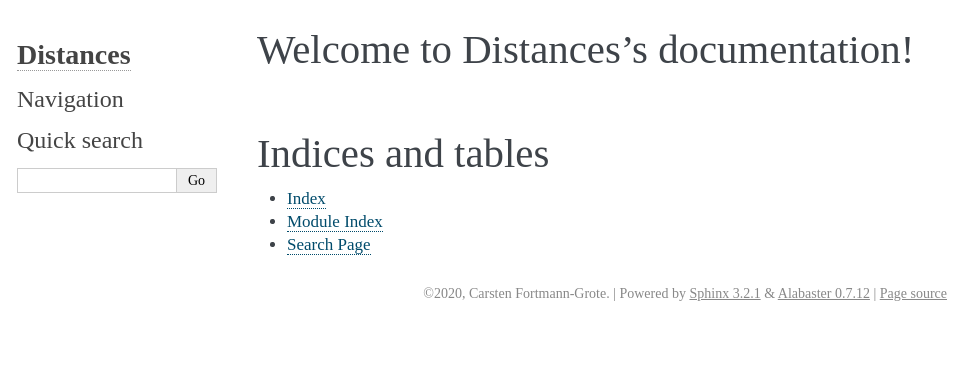
\includegraphics{static/docs_header.png}
\caption{Screenshot\_2020-12-08\_10-35-20.png}
\end{figure}

\hypertarget{adding-the-documentation-content}{%
\subsection{Adding the documentation
content}\label{adding-the-documentation-content}}

Now it's time to add some content to our documentation and link in the
docstrings from the code.

The file \texttt{doc/source/index.rst} is the root document of the
documentation. It is formatted in the \texttt{ReStructuredText} markup
language. E.g. top level headings are underlined by \texttt{===},
directives start with \texttt{..} and so on. See the
\href{https://www.sphinx-doc.org/en/master/usage/restructuredtext/basics.html}{ReStructuredText
manual} for details. To add our modules' documentation, we first have to
convert their docstrings into \texttt{ReStructuredText}: From the
\texttt{doc/} directory, run

\begin{verbatim}
$ sphinx-apidoc -f -o source ../distances
\end{verbatim}

This will create two new files in the \texttt{source/} directory,
\texttt{modules.rst} and \texttt{distances.rst}. These contain the
formatted version of our docstrings. Now, we can easily include the
distances documentation in the \texttt{index.rst} by adding one line
after the \texttt{..\ toctree} directive. Your \texttt{index.rst} should
look like this:

\begin{Shaded}
\begin{Highlighting}[]
\CommentTok{.. doc/source/index.rst}

\NormalTok{Welcome to Distances\textquotesingle{}s documentation!}
\NormalTok{=====================================}

\DataTypeTok{.. toctree::}
   \FunctionTok{:maxdepth:}\NormalTok{ 2}
   \FunctionTok{:caption:}\NormalTok{ Contents:}

\NormalTok{   distances}


\NormalTok{Indices and tables}
\NormalTok{==================}

\NormalTok{* }\KeywordTok{:ref:}\DecValTok{\textasciigrave{}genindex\textasciigrave{}}
\NormalTok{* }\KeywordTok{:ref:}\DecValTok{\textasciigrave{}modindex\textasciigrave{}}
\NormalTok{* }\KeywordTok{:ref:}\DecValTok{\textasciigrave{}search\textasciigrave{}}
\end{Highlighting}
\end{Shaded}

Build the documentation again:

\begin{verbatim}
$ make html
\end{verbatim}

Reload the documentation website at http://localhost:8000 (supposing
that the webserver is still running, otherwise restart it,
Section \ref{python_web_server}).

You should now see a beautiful documentation website similar to this
one:

\begin{figure}
\centering
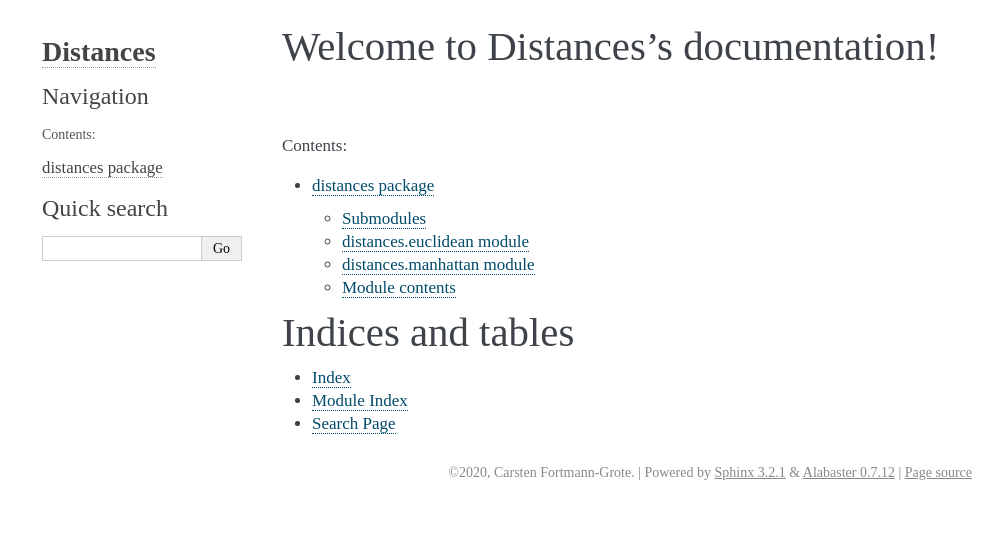
\includegraphics{static/docs.png}
\caption{Screenshot\_2020-12-08\_11-12-51.png}
\end{figure}

Take some time to browse around your documentation site and try to
mentally connect the contents of the \texttt{.rst} files and the
elements and links in the webpage.

    \hypertarget{let-gitlab-ci-build-the-documentation-gitlab-pages}{%
\subsection{Let gitlab-CI build the documentation:
gitlab-pages}\label{let-gitlab-ci-build-the-documentation-gitlab-pages}}

So far we have \emph{manually} built the documentation. What we want is
that each time the code and/or the documentation changes, the manual is
rebuilt to reflect these changes. We need to define a new CI job in our
pipeline.

Change back to the repository root directory and edit the file
\texttt{.gitlab-ci.yml}.

\begin{Shaded}
\begin{Highlighting}[]
\CommentTok{\# gitlab{-}ci yaml file for project "distances"}
\CommentTok{\# The docker base image to use.}
\FunctionTok{image}\KeywordTok{:}\AttributeTok{ python:latest}

\CommentTok{\# Run these commands before any jobs.}
\FunctionTok{before\_script}\KeywordTok{:}
\AttributeTok{  }\KeywordTok{{-}}\AttributeTok{ python {-}V}\CommentTok{                 \# Print out python version for debugging}
\AttributeTok{  }\KeywordTok{{-}}\AttributeTok{ pip install virtualenv}\CommentTok{    \# Pip install dependencies}
\AttributeTok{  }\KeywordTok{{-}}\AttributeTok{ virtualenv venv}\CommentTok{           \# Create }
\AttributeTok{  }\KeywordTok{{-}}\AttributeTok{ source venv/bin/activate}\CommentTok{  \# Activate the virtual environment.}
\AttributeTok{  }\KeywordTok{{-}}\AttributeTok{ pip install pytest}\CommentTok{        \# Install pytest into the venv.}
\AttributeTok{  }\KeywordTok{{-}}\AttributeTok{ pip install sphinx}\CommentTok{        \# Install pytest into the venv.}

\CommentTok{\# The test job }
\FunctionTok{test}\KeywordTok{:}
\AttributeTok{  }\FunctionTok{script}\KeywordTok{:}
\AttributeTok{    }\KeywordTok{{-}}\AttributeTok{ pytest test\_euclidean.py}
\AttributeTok{    }\KeywordTok{{-}}\AttributeTok{ pytest test\_manhattan.py}

\FunctionTok{pages}\KeywordTok{:}
\AttributeTok{  }\FunctionTok{script}\KeywordTok{:}
\AttributeTok{    }\KeywordTok{{-}}\AttributeTok{ cd doc}
\AttributeTok{    }\KeywordTok{{-}}\AttributeTok{ sphinx{-}apidoc {-}f {-}o source ../distances}
\AttributeTok{    }\KeywordTok{{-}}\AttributeTok{ make html}
\AttributeTok{    }\KeywordTok{{-}}\AttributeTok{ cp {-}av build/html ../public}
\AttributeTok{  }\FunctionTok{artifacts}\KeywordTok{:}
\AttributeTok{    }\FunctionTok{paths}\KeywordTok{:}
\AttributeTok{      }\KeywordTok{{-}}\AttributeTok{ public}
\end{Highlighting}
\end{Shaded}

We add the \texttt{pages} job at the end. It contains all steps to take
to build the documentation. The last step is to copy the built
documentation website to a directory \texttt{pages} under the repository
root. The \texttt{artifacts} directive ensures that the \texttt{public}
directory will be maintained when the site is exposed through a
webserver.

\hypertarget{push-to-gitlab}{%
\subsection{Push to gitlab}\label{push-to-gitlab}}

We have now configured our repository to automatically build the
reference manual. Let's add all needed new files to git and push to
gitlab.

\begin{verbatim}
$ git add doc/Makefile
$ git add doc/make.bat
$ git add doc/source/conf.py
$ git add doc/source/index.rst
$ git add .gitlab-ci.yml

$ git commit
$ git push -u origin doc
\end{verbatim}

The last command pushes our changes to a new remote branch \texttt{doc}.

Observe the status of your CI pipeline under CI/CD -\textgreater{}
Pipelines. Note that the pipeline now contains two Jobs, one for testing
and one for building the documentation. After the second job succeeds,
you should be able to open your online documentation site at
http://.pages.gwdg.de/distances.

\hypertarget{build-documentation-only-for-the-master-branch}{%
\subsection{Build documentation only for the master
branch}\label{build-documentation-only-for-the-master-branch}}

To make sure that the documentation is built only on the master branch,
we add one more directive to \texttt{.gitlab-ci.yml}:

\begin{Shaded}
\begin{Highlighting}[]
\CommentTok{\# gitlab{-}ci yaml file for project "distances"}
\CommentTok{\# The docker base image to use.}
\FunctionTok{image}\KeywordTok{:}\AttributeTok{ python:latest}

\CommentTok{\# Run these commands before any jobs.}
\FunctionTok{before\_script}\KeywordTok{:}
\AttributeTok{  }\KeywordTok{{-}}\AttributeTok{ python {-}V}\CommentTok{                 \# Print out python version for debugging}
\AttributeTok{  }\KeywordTok{{-}}\AttributeTok{ pip install virtualenv}\CommentTok{    \# Pip install dependencies}
\AttributeTok{  }\KeywordTok{{-}}\AttributeTok{ virtualenv venv}\CommentTok{           \# Create }
\AttributeTok{  }\KeywordTok{{-}}\AttributeTok{ source venv/bin/activate}\CommentTok{  \# Activate the virtual environment.}
\AttributeTok{  }\KeywordTok{{-}}\AttributeTok{ pip install pytest}\CommentTok{        \# Install pytest into the venv.}
\AttributeTok{  }\KeywordTok{{-}}\AttributeTok{ pip install sphinx}\CommentTok{        \# Install pytest into the venv.}

\CommentTok{\# The test job }
\FunctionTok{test}\KeywordTok{:}
\AttributeTok{  }\FunctionTok{script}\KeywordTok{:}
\AttributeTok{    }\KeywordTok{{-}}\AttributeTok{ pytest test\_euclidean.py}
\AttributeTok{    }\KeywordTok{{-}}\AttributeTok{ pytest test\_manhattan.py}

\FunctionTok{pages}\KeywordTok{:}
\AttributeTok{  }\FunctionTok{script}\KeywordTok{:}
\AttributeTok{    }\KeywordTok{{-}}\AttributeTok{ cd doc}
\AttributeTok{    }\KeywordTok{{-}}\AttributeTok{ sphinx{-}apidoc {-}f {-}o source ../distances}
\AttributeTok{    }\KeywordTok{{-}}\AttributeTok{ make html}
\AttributeTok{    }\KeywordTok{{-}}\AttributeTok{ cp {-}av build/html ../public}
\AttributeTok{  }\FunctionTok{artifacts}\KeywordTok{:}
\AttributeTok{    }\FunctionTok{paths}\KeywordTok{:}
\AttributeTok{      }\KeywordTok{{-}}\AttributeTok{ public}
\AttributeTok{  }\FunctionTok{only}\KeywordTok{:}
\AttributeTok{    }\KeywordTok{{-}}\AttributeTok{ master}
\end{Highlighting}
\end{Shaded}

Add, commit, and push again and then create a merge request to merge the
\texttt{doc} branch into \texttt{master}. Note that the CI pipeline is
also run on the Merge request, so you can detect possible issues already
before the final merge.

    \hypertarget{add-test-and-documentation-badges-to-readme}{%
\subsection{Add test and documentation badges to
README}\label{add-test-and-documentation-badges-to-readme}}

    As a final gimmick, let's be hip and show off our test status on the
repository's front page. Follow these steps:

\begin{itemize}
\tightlist
\item
  Navigate to your project's Settings \textgreater{} General
  \textgreater{} Badges.
\item
  Under Name, enter Pipeline Status.
\item
  Under Link, enter the following URL:
  https://gitlab.com/\%\{project\_path\}/-/commits/\%\{default\_branch\}
\item
  Under Badge image URL, enter the following URL:
  https://gitlab.com/\%\{project\_path\}/badges/\%\{default\_branch\}/pipeline.svg
\item
  Submit the badge by clicking the Add badge button.
\end{itemize}

The pipeline status badge will then appear on top of the repository's
front page:

    \begin{tcolorbox}[breakable, size=fbox, boxrule=1pt, pad at break*=1mm,colback=cellbackground, colframe=cellborder]
\prompt{In}{incolor}{ }{\boxspacing}
\begin{Verbatim}[commandchars=\\\{\}]

\end{Verbatim}
\end{tcolorbox}


    % Add a bibliography block to the postdoc
    
    
    
\end{document}
